\section*{Results}

	\subsection*{Clustering of the food webs}

		The 86 food webs had a median of 25.5 nodes (IQR = 16.0), with a minimum of 14 nodes and a maximum of 55 nodes. See Figure \ref{fig:food_web_sizes}. They produced a median number of 0.76 (IQR = 0.11) for the Jaccard index, 0.73 (IQR = 0.07) for the REGE index, 0.16 (IQR = 0.08) for the density modularity, 0.35 (IQR = 0.02) for the prey modularity, 0.16 (IQR = 0.08) for the predator modularity and 0.16 (IQR = 0.07) for the group model. See Figure \ref{fig:cluster_sizes}.

						\begin{figure}[htbp]%{\textwidth}
								\centering
								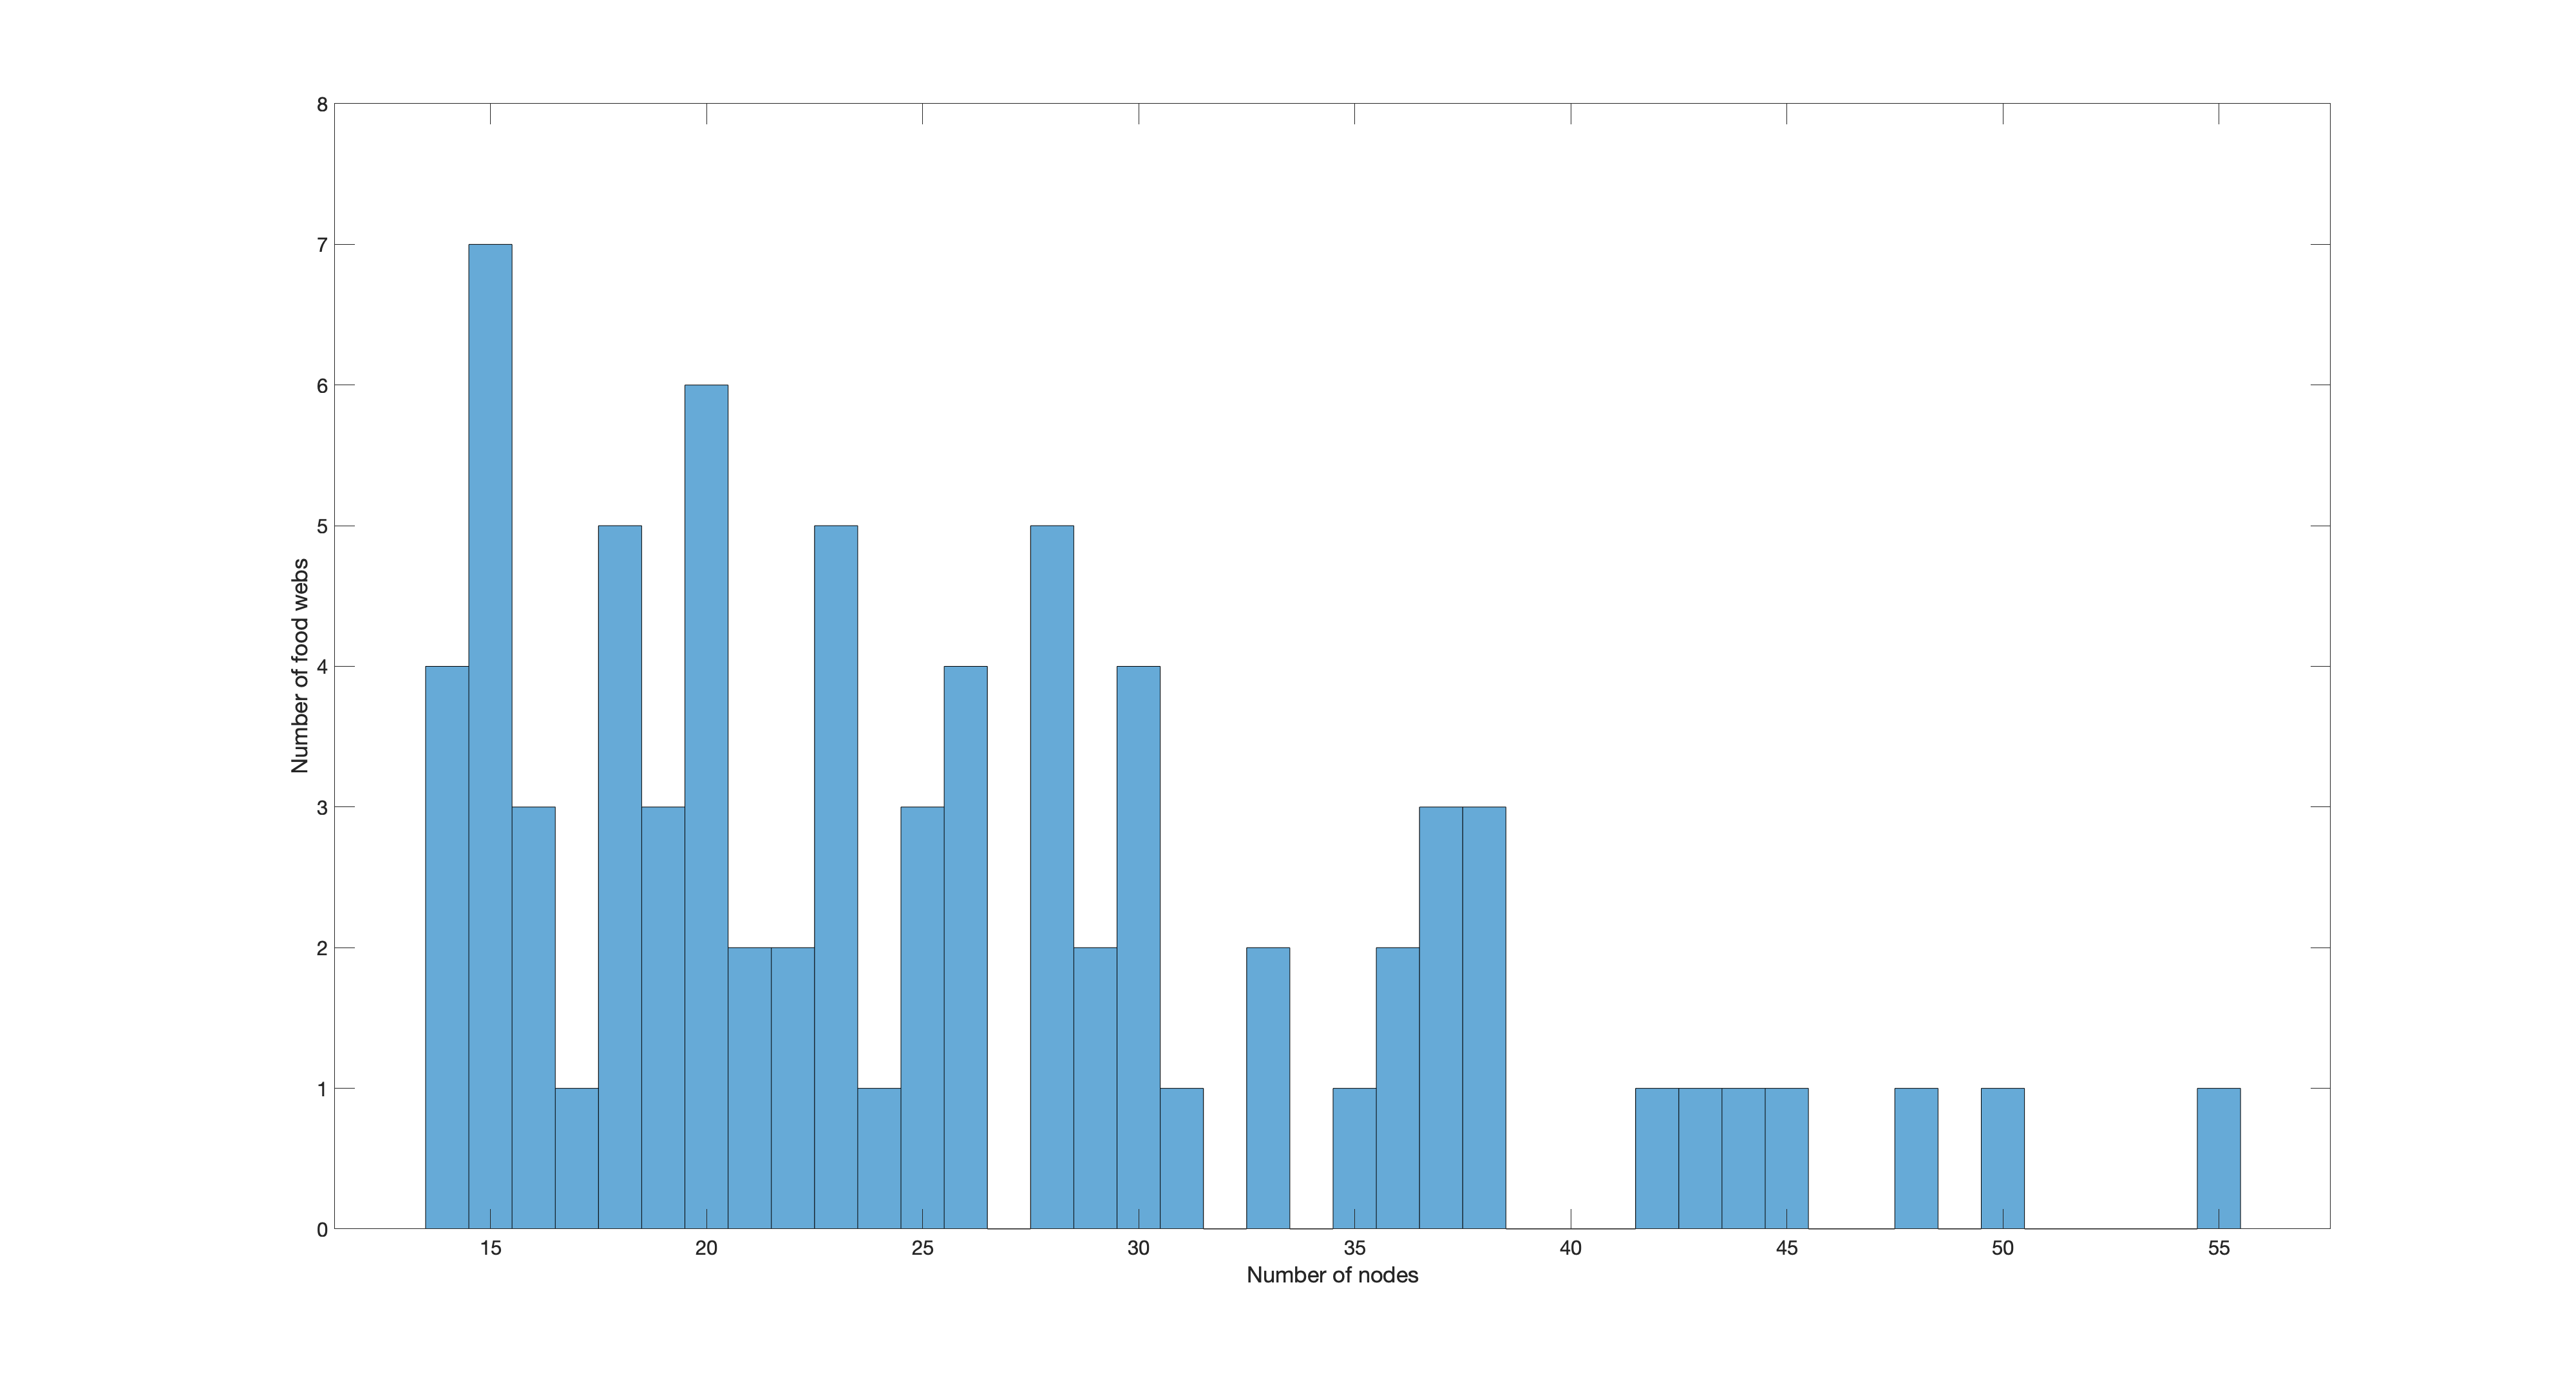
\includegraphics[width=1.0 \linewidth]{food_web_sizes.jpg}
								\caption{Size of the 86 food webs used in this study.}
								\label{fig:food_web_sizes}
						\end{figure}

						\begin{figure}[htbp]%{\textwidth}
								\centering
								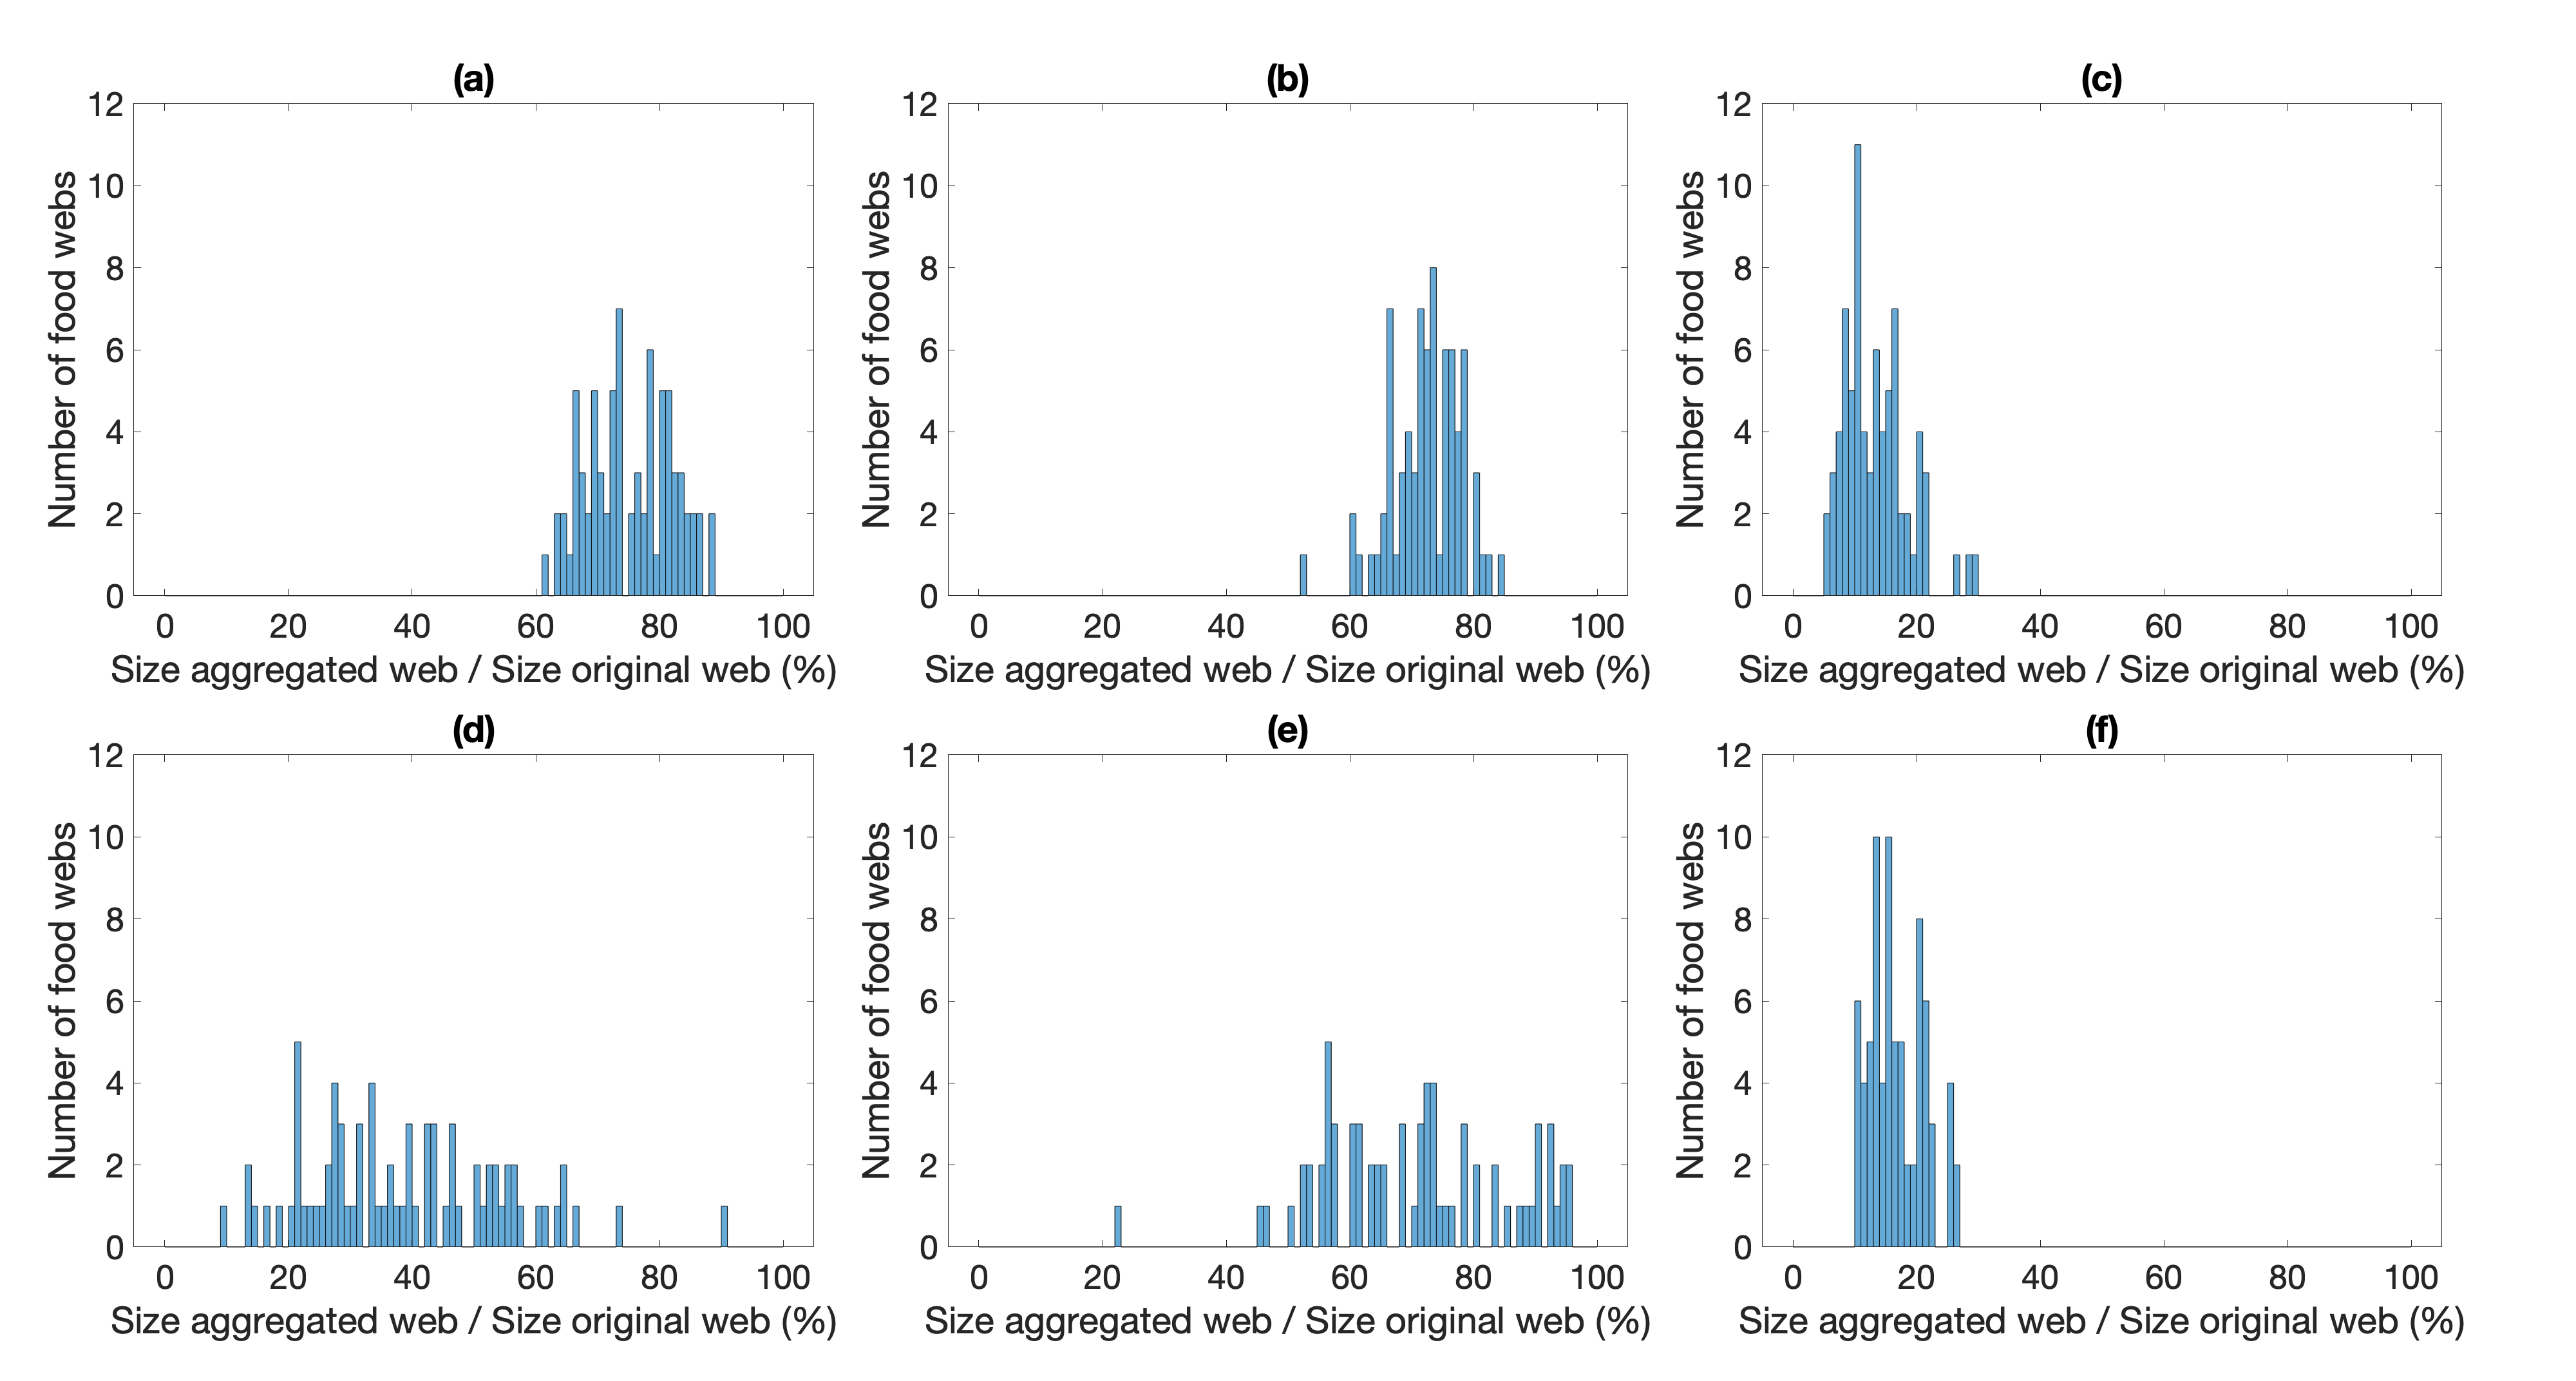
\includegraphics[width=1.0\linewidth]{cluster_sizes.jpg}
								\caption{Number of clusters produced by the different aggregation methods. (a) = hierarchical clustering with Jaccard index, (b) = hierarchical clustering with REGE index, (c) = density-based modules, (d) = prey-based modules, (e) = predator-based modules, (f) = groups.}
								\label{fig:cluster_sizes}
							\end{figure}


	\subsection*{Comparison between the original and the clustered rankings}

	The results of the comparison between the ranking of nodes in the original and the clustered food webs can be seen in Figure \ref{fig:jaccard_results} - \ref{fig:groups_results}.
